\documentclass[border=3pt]{standalone}
\usepackage{times}
\usepackage{amsmath,bm}
\usepackage{tikz}
\usetikzlibrary{positioning,arrows.meta,fit,calc}
\begin{document}
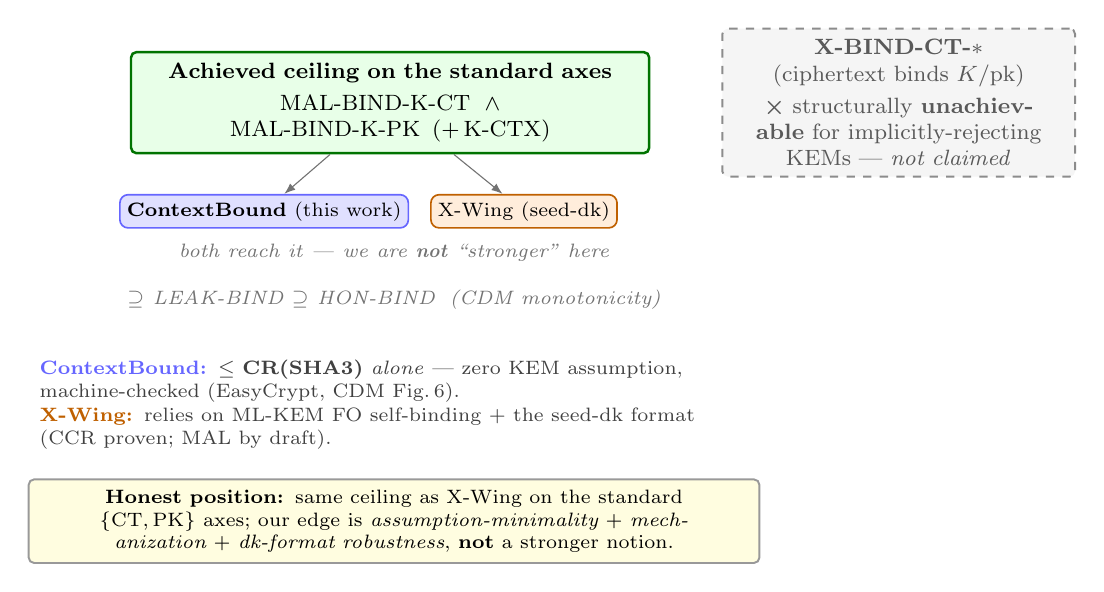
\begin{tikzpicture}[
  font=\footnotesize, >={Latex[length=4pt]},
  box/.style={draw, rounded corners=2pt, align=center, inner sep=4pt, line width=0.7pt},
  ceil/.style={box, fill=green!9, draw=green!45!black, line width=0.9pt},
  chip/.style={draw, rounded corners=3pt, inner sep=2.5pt, font=\scriptsize, line width=0.6pt},
  na/.style={box, fill=black!4, draw=black!45, dashed, text=black!65},
  note/.style={font=\scriptsize, align=left, text=black!75},
  lbl/.style={font=\scriptsize\itshape, text=black!55, align=center},
]
% ---- achieved ceiling ----
\node[ceil, text width=63mm] (ceil)
  {\textbf{Achieved ceiling on the standard axes}\\[2pt]
   \mbox{MAL-BIND-K-CT} \;$\wedge$\; \mbox{MAL-BIND-K-PK} \,($+$\,K-CTX)};
% ---- the two schemes (chips) ----
\node[chip, fill=blue!12, draw=blue!60, below=5mm of ceil, xshift=-16mm] (cb)
  {\textbf{ContextBound} (this work)};
\node[chip, fill=orange!14, draw=orange!75!black, below=5mm of ceil, xshift=17mm] (xw)
  {X-Wing (seed-dk)};
\draw[->, black!55] (ceil) -- (cb);
\draw[->, black!55] (ceil) -- (xw);
% ---- chained notes, centred under the chips ----
\node[lbl] (br) at ($(cb.south)!0.5!(xw.south)+(0,-3mm)$)
  {both reach it --- we are \textbf{not} ``stronger'' here};
\node[lbl, below=1.2mm of br] (mono)
  {$\supseteq$ LEAK-BIND $\supseteq$ HON-BIND \;(CDM monotonicity)};
\node[note, below=4mm of mono, text width=90mm] (asm)
  {\textcolor{blue!60}{\textbf{ContextBound:}} $\le$ \textbf{CR(SHA3)} \emph{alone} --- zero KEM assumption,
   machine-checked (EasyCrypt, CDM Fig.\,6).\\[1pt]
   \textcolor{orange!75!black}{\textbf{X-Wing:}} relies on ML-KEM FO self-binding $+$ the seed-dk format
   (CCR proven; MAL by draft).};
\node[box, below=2.5mm of asm, fill=yellow!12, draw=black!40, text width=90mm, font=\scriptsize] (take)
  {\textbf{Honest position:} same ceiling as X-Wing on the standard \{CT,\,PK\} axes; our edge is
   \emph{assumption-minimality $+$ mechanization $+$ dk-format robustness}, \textbf{not} a stronger notion.};
% ---- unachievable region (top right) ----
\node[na, right=9mm of ceil, text width=42mm] (na)
  {\textbf{X-BIND-CT-$\ast$} \;(ciphertext binds $K$/pk)\\[2pt]
   $\bm{\times}$ structurally \textbf{unachievable} for implicitly-rejecting KEMs --- \emph{not claimed}};
\end{tikzpicture}
\end{document}
